\newpage
\section{Lights and rendering}
To obtain realistic images with filled 3D primitives, \textbf{light reflection} should be correctly emulated.Some definitions:
\begin{itemize}
\item \textbf{Rendering} reproduces the effects of the illumination by defining light sources and surface properties. 
\item \textbf{Lights} are the sources of illumination ,used to makes objects visible
\item \textbf{Materials} set the parameters that determine how light is reflected.
\end{itemize}
The algorithms used to compute the colors of a surface starting from lights and material are called \textbf{Shaders}.\\
As seen in Chap.1 light sources emit different frequencies of the spectrum and objects \textbf{reflect} part of them. The photons emitted by the lights source bounce of the objects and some of them reach the viewpoint (camera) : rendering computes the \textbf{quantity} and the \textbf{color} of such photons.
\begin{figure}[H]
  \centering
  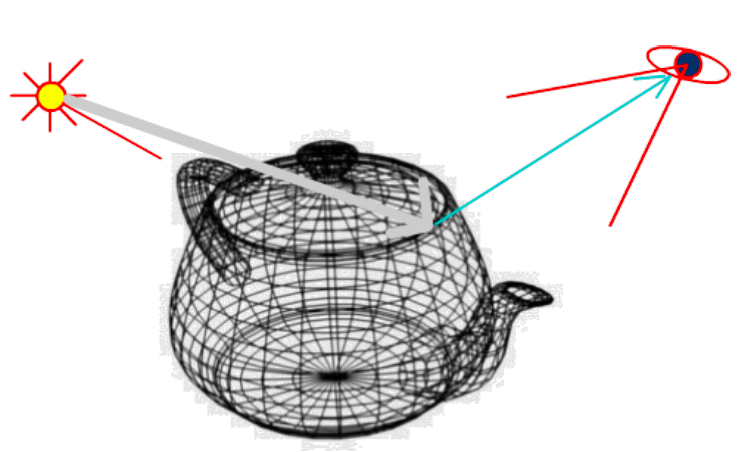
\includegraphics[width=.4\linewidth]{reflection}
\end{figure}

\subsection{The Bidirectional Reflectance Distribution Function}
Rendering must be able to define the \textbf{radiance} (quantity of light) received in each point of the projection plane ( each pixel) according to the direction of the corresponding projection ray.The \textbf{direction} and \textbf{intensity} of reflection is determined by the material that compose the surface of an object : 
the direction bounce depends on the microscopic structure of the surface
\begin{figure}[H]
  \centering
  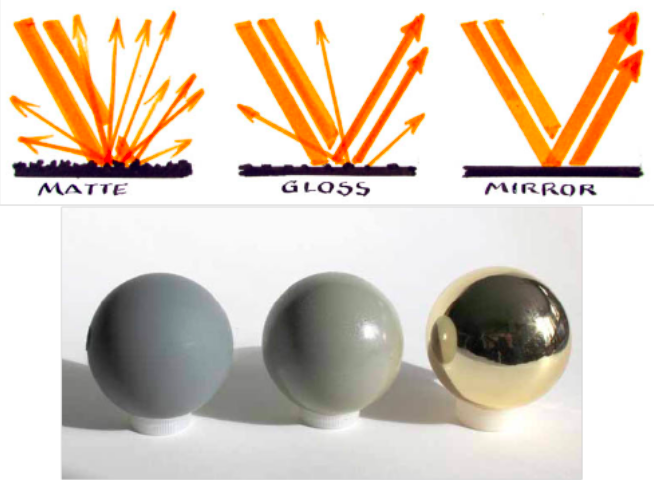
\includegraphics[width=.4\linewidth]{materials}
\end{figure}
These surface properties can be encoded by the \textbf{bidirectional reflectance distribution function (BRDF)}
\begin{figure}[H]
  \centering
  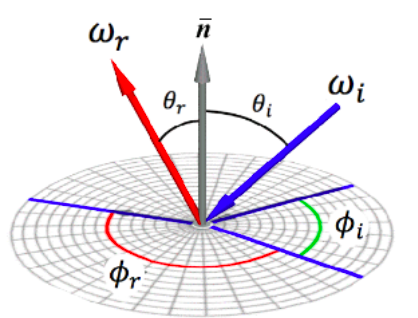
\includegraphics[width=.4\linewidth]{brdf}
\end{figure}
The inputs of the function are $\omega_i$ (direction of incoming light) and $\omega_r$ (direction that tells us if the objects reflects or not light in that direction). The output is the probability of reflecting in direction $\omega_r$ coming from $\omega_i$. In the case of a \textbf{mirror} surface, the probability will be equal to 0 for all $\omega_r$ except the one corresponding to angle $\theta_r = \theta_i$. $$ f_r(\theta_i,\phi_i,\theta_r,\phi_r)= f_r(\omega_i,\omega_r)$$
This function allows considering different ways in which the incoming radiance can be reflected at different angles,depending on the material.
The BRDF function is expressed as sum of two terms:
\begin{itemize}
\item the \textbf{diffuse reflection}\\
Represents the main color of the object 
\begin{figure}[H]
  \centering
  
\includegraphics[width=.4\linewidth]{diffuse}
\end{figure}
\item the \textbf{specular reflection}\\
Shiny objects tend to reflect the incoming light in a particular angle called the specular direction
\begin{figure}[H]
  \centering
  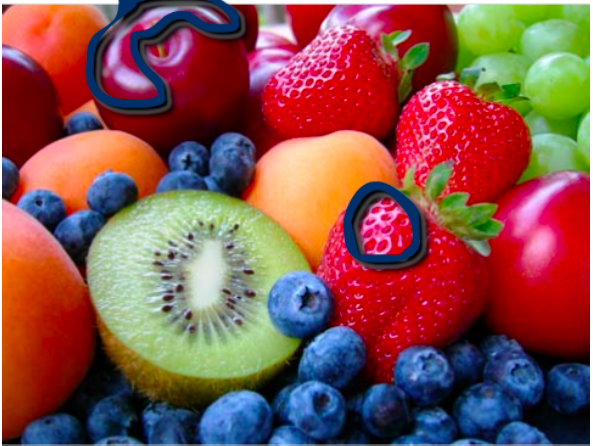
\includegraphics[width=.4\linewidth]{specular}
\end{figure}
\end{itemize}
$$ f_r(x,\vec{lx},\omega_r)= f_{diffuse}(x,\vec{lx},\omega_r)+f_{specular}(x,\vec{lx},\omega_r)$$
\subsection{Rendering equation}
The BRDF allows relating together the irradiance in all the directions for all points in a scene in the so called \textbf{rendering equation}:
$$ L(x,\omega_r)= L_e(x,\omega_r)+ \int {L(y,\vec{yx})f_r(x,\vec{yx},\omega_r)G(x,y)V(x,y)dy}$$
This is a very complex equation but a simplified equation is available  : the \textbf{scan-line rendering equation}. The approximation that is done is that only a specific \textbf{finite} set of lights sources illuminate the scene (sum over l light sources). The contributions of each light source l to the final color of the pixel are added together. Each term is determined as the product of :
\begin{itemize}
\item the \textbf{light model} : quantity and direction of the light source. Vector $\vec{lx}$ connect the light l to the point x.
\item the \textbf{BRDF} of the surface that reflects the light
\end{itemize}
\[
\boxed{L(x,\omega_r) = \sum\limits_{l}L(l,\vec{lx})f_r(x,\vec{lx},\omega_r)}
\]
This equation tells the total radiance of point \textbf{x} of an object in a direction $\omega_r$ of the space.
\begin{figure}[H]
  \centering
  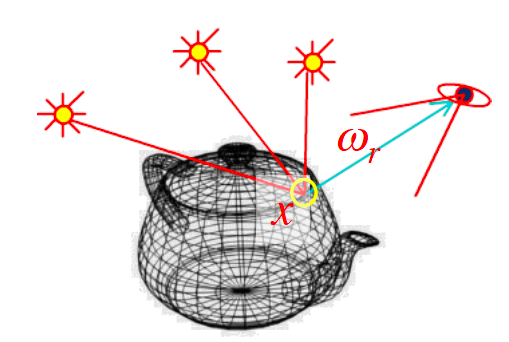
\includegraphics[width=.4\linewidth]{scanline}
\end{figure}

\subsubsection{Scan-line : considering colors}
The scan-line equation should be repeated for \textbf{every wavelength} of the light (the three different RGB channels): $$ L(x,\omega_r,\lambda) = \sum\limits_{l}L(l,\vec{lx},\lambda)f_r(x,\vec{lx},\omega_r,\lambda)$$
The lights have associated RGB values that accounts for the photons emitted for each of the three main frequencies.Objects are characterized by a different BRDF for each of the three main frequencies : three separate images are produced independently and summed up to produce the final image.\\
Due to the separation of color components , combinations of lights and material colors can lead to unexpected results :
\begin{figure}[H]
  \centering
  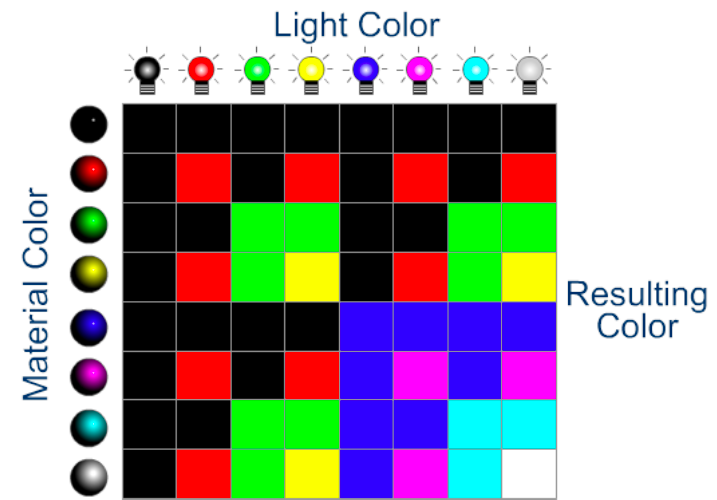
\includegraphics[width=.4\linewidth]{colorcomb}
\end{figure}
For example purple light illuminating a yellow objects results in a red color. This is because in the scan-line equation one of the terms is equal to zero .\\
In the scan-line rendering equation all terms are $\in [0,1]$ range. It can happen that the sum of the terms $\sum\limits_{l}L(l,\vec{lx})f_r(x,\vec{lx},\omega_r) >1$. To solve this \textbf{clamping} is applied :
\[
\boxed{L(x,\omega_r)= \text{clamp} \left( \sum\limits_{l}L(l,\vec{lx})f_r(x,\vec{lx},\omega_r) \right) }
\]


\[ clamp =
  \begin{cases}
    0       & \quad y<0\\
    y  & \quad y \in [0,1]\\
    1  & \quad y >1
  \end{cases}
\]
This effect can be seen in overexposed images : areas that contain RGB values greater than 1 will be clamped to be 1. So for example $(7.3,2.5,1.6)$ after clamping becomes $(1,1,1)$ which translates to the \textbf{white color} , characteristic of overexposed photos.

\subsection{Light models}
Here are considered three different light models that describe how light is emitted in different \textbf{directions} of the space and at which \textbf{intensity}. 

\subsubsection{Direct light models}
Direction or direct lights are sources of light that are \textbf{far away} from the objects (for example the sun in a scene). Due to the distance of the source the light rays are \textbf{parallel} to each other in all the positions of the space.
\begin{figure}[H]
  \centering
  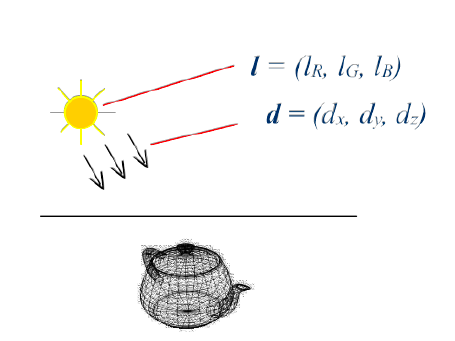
\includegraphics[width=.4\linewidth]{directl}
\end{figure}
\begin{itemize}
\item $d=(d_x,d_y,d_z)$ specifies the \textbf{light direction} that is independent of the position of the objects in the scene ($ \vec{lx} = d$).Conventionally the direction vector d is unitary ($|d|=1$) and is pointing \textbf{from } the object \textbf{to} the light
\begin{figure}[H]
  \centering
  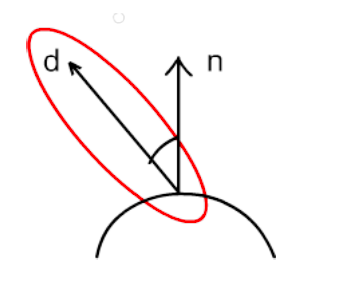
\includegraphics[width=.4\linewidth]{directl2}
\end{figure}
\item $l=(l_R,l_G,l_B)$ is the RGB component vector that defines the light color.Since the quantity of light emitted per direction is the same, all parts of the scene receive the same amount of red, green and blue.This means the $L(l,\vec{lx}) = l$
\end{itemize}
So the scan-line equation becomes :
\[
\boxed{L(x,\omega_r)= l * f_r(x,d,\omega_r)}
\]
The star * indicates the element wise product of the terms ( l is a vector of colors , and the BRDF returns also a vector) since we are not considering the single color frequencies $\lambda$.

\subsubsection{Point Lights}
Point lights emit light from a \textbf{fixed} position in space characterized by their position. Rotating the light while maintaining the position does not alter the scene (like a lamp in a room) : they emit light in all the directions, starting from a specific position in space.
\begin{itemize}
\item $p=(p_x,p_y,p_z)$ position of point light
\item $l=(l_R,l_G,l_B)$ color vector
\item the direction (required by BRDF) varies according to the point \textbf{x} of the object that is illuminated  $$ \vec{lx} = \frac{p-x}{|p-x|}$$The vector is normalized to make the vector unitary.
\end{itemize}
To reproduce the physical properties of light sources, point lights are characterized by a \textbf{decay factor} : the intensity of a point light reduces at a rate that is proportional to the\textbf{ inverse of the square of the distance}
\begin{figure}[H]
  \centering
  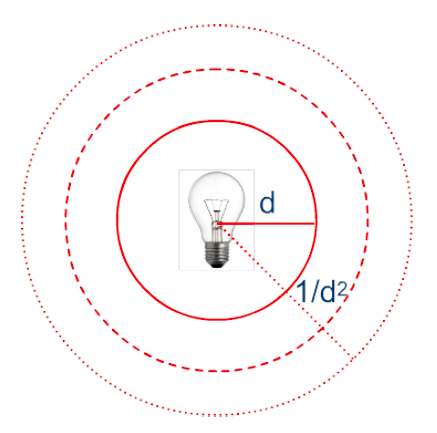
\includegraphics[width=.4\linewidth]{pointl}
\end{figure}
Implementing this results in images that often are very dark as the light does not bounce of the other objects resulting in a more illuminated area. This is where the \textbf{decay factor} $\beta$ comes in handy. Another parameter that increases physical behaviour is the \textbf{scaling factor g}.
\[
\boxed{L(l,\vec{lx})= l \left( \frac{g}{|p-x|} \right)^{\beta}}
\]
\begin{itemize}
\item $\beta=0 \to$ constant light without decay.
\item $\beta=1 \to$ inverse linear decay
\item $\beta=2 \to$ inverse squared decay (most like in reality) 
\end{itemize}
The scan-line rendering equation becomes (with decay) :
\[
\boxed{L(x,\omega_r)= l \left( \frac{g}{|p-x|} \right)^{\beta} * f_r \left( x, \frac{p-x}{|p-x|},\omega_r \right)}
\]
The scan-line rendering equation becomes (without decay) :
\[
\boxed{L(x,\omega_r)= l* f_r \left( x, \frac{p-x}{|p-x|},\omega_r \right )}
\]

\subsubsection{Spot lights}
Spot lights are light sources characterized by a \textbf{position p } from where they emit in a \textbf{distance d}.
\begin{figure}[H]
  \centering
  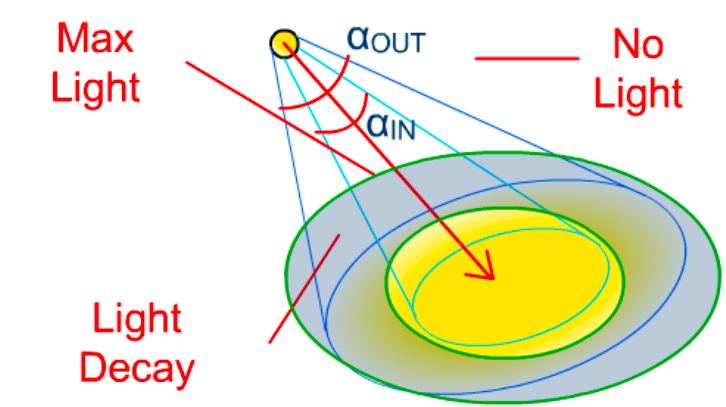
\includegraphics[width=.4\linewidth]{spotl}
\end{figure}
Spotlights divide the scene into three area : 
\begin{itemize}
\item where direct light (max light) is received ( $< \alpha_{IN}$ )
\item where decaying light is received ($> \alpha_{IN} , < \alpha_{OUT}$)
\item where no light is received  ($>\alpha_{OUT}$)
\end{itemize}
The closer the two angles are together the clearer is the cut . The more they are fare away the more the light is faded.\\
Since the spotlight is an extension of the point light it is characterized by the same color vector \textbf{l} and the \textbf{decay factor} $\beta$. For the implementation of the spotlight usually the \textbf{cosine} of the half-angles are used ( $c_{IN} > c_{OUT}$ ) 
\begin{figure}[H]
  \centering
  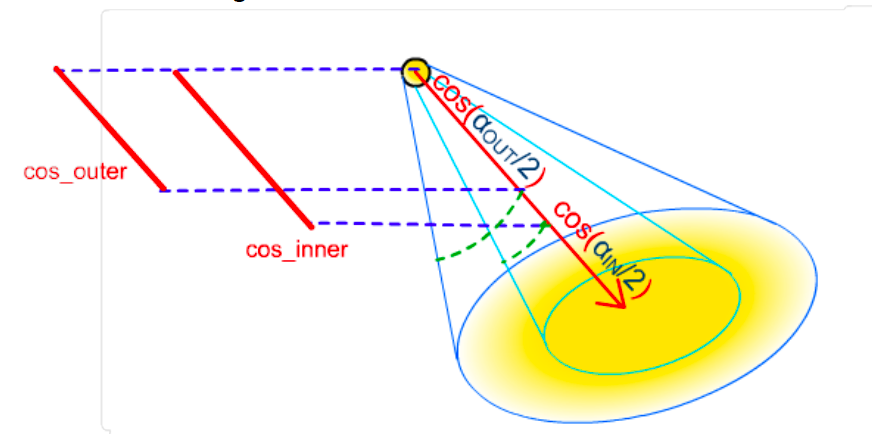
\includegraphics[width=.4\linewidth]{spotl2}
\end{figure}
Computing $$ cos \alpha_{l} = \vec{lx} \cdot d$$ where $\alpha_l$ is the angle formed by the vector from the center of the light to the point x.
By applying clamping the \textbf{cone } of light is computed as:
$$ \text{clamp} \left( \frac{cos\alpha_l - c_{out}}{c_{IN}-c_{OUT}} \right)$$
The scan-line equation becomes (with decay):
\[
\boxed{L(x,\omega_r)= l \left( \frac{g}{|p-x|} \right)^{\beta} \cdot \text{clamp} \left( \frac{\frac{p-x}{|p-x|} \cdot d  - c_{out}}{c_{IN}-c_{OUT}} \right) * f_r \left( x, \frac{p-x}{|p-x|},\omega_r \right) }
\]
The scan-line equation becomes (without decay):
\[
\boxed{L(x,\omega_r)= l \cdot \text{clamp} \left( \frac{\frac{p-x}{|p-x|} \cdot d - c_{out}}{c_{IN}-c_{OUT}} \right) * f_r \left( x, \frac{p-x}{|p-x|},\omega_r \right) }
\]


\subsection{BRDF Models}
Here are considered three different BRDF models that describe how much light is reflected off the surface of an object. As already seen the BRDF is composed of two terms, the \textbf{diffuse} and the \textbf{specular} term. The \textbf{Lambert Model} refers to the diffuse part and the \textbf{Phong} and \textbf{Blinn} refer to the specular part.

\subsubsection{Diffuse: Lambert Model} 
The Lambert Model would be enough to render the color of an object but it would appear \textbf{matt} (no \textbf{specular} part). The \textbf{Lambert reflection law} states that each point that is hit by a light ray,reflect it with \textbf{uniform probability} in \textbf{all} directions. The reflection is \textbf{independent} of the viewing angle and corresponds to a \textbf{constant} BRDF : 
$$ f_r(x,\omega_i,\omega_r)=\rho_x$$
\begin{figure}[H]
  \centering
  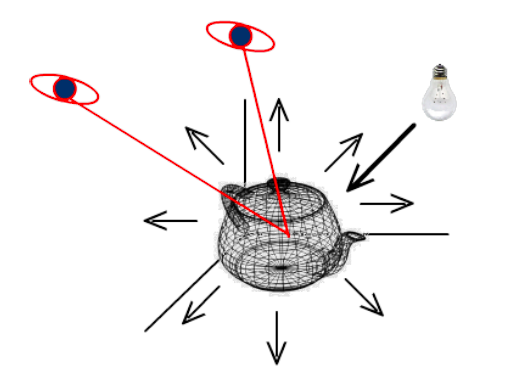
\includegraphics[width=.4\linewidth]{lambert}
\end{figure}
However the \textbf{quantity} of light received by an object, depends on the \textbf{angle} between the ray of light and the reflecting surface. Consider $n_x$ being the normal (normalized) vector to the surface, $d$ the direction of the ray of light  of unitary length directed from the object to the source of light ( convention) :
\begin{figure}[H]
  \centering
  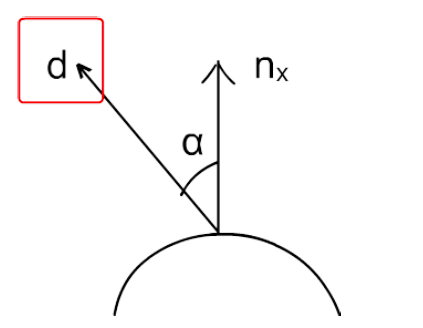
\includegraphics[width=.4\linewidth]{lambert2}
\end{figure}
This way the amount of received light can be described :
\begin{figure}[H]
  \centering
  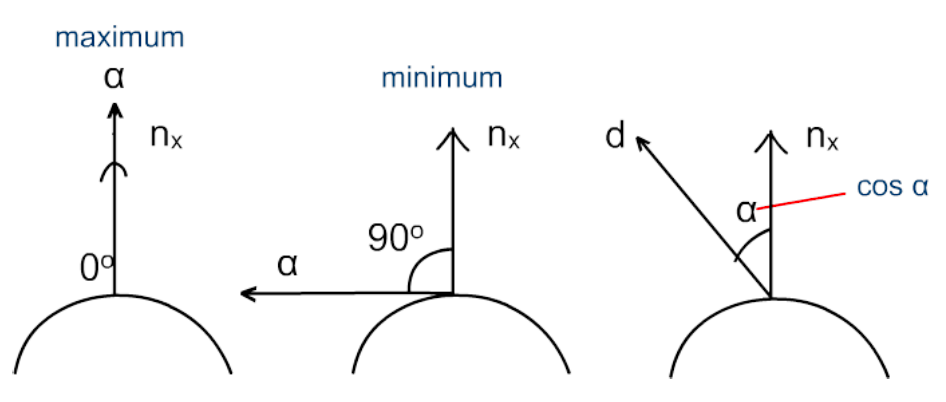
\includegraphics[width=.5\linewidth]{lambert3}
\end{figure}
As seen in the figure Lambert found out that the amount of light is proportional to the cosine of the angle between the direction of the light and the normal to the surface: $$ \vec{d} \cdot \vec{n_x} = cos\alpha$$
Next the behaviour of the BRDF function with respect to a specific color must be analysed . The vector $$ m_D = (m_R,m_G,m_B)$$ (\textbf{diffuse color}) expresses the capability of a material to perform  the Lambert reflection for each of the three primary color frequencies RGB (so $\rho_x = m_D$	, the constant assigned to the BRDF). This tell how each frequency is reflected by the object.
The diffuse part of the BRDF becomes :
\[
\boxed{f_r(x,\vec{lx},\omega_r)=f_{diffuse}=m_D \cdot \text{clamp}(\vec{lx} \cdot n_x)}
\]
The clamp function limits the scalar product in range [0,1] instead of [-1,1]. Normally if the cosine of the angle is -1 then we're referring to the backface of the object which will be excluded by back-face culling. It is still good practice to set the received light to 0.\\
Point light (no decay )model example :
$$ L(x,\omega_r) = l * m_D \cdot \text{clamp} \left( \frac{p-x}{|p-x|} \cdot n_x \right)$$
Directional light model example :
$$ L(x,\omega_r) = l * m_D \cdot \text{clamp} \left( d \cdot n_x \right)$$

\subsubsection{Specular: Phong Model and Blinn Model} 
Most of the materials reflect more than the incoming light in the specular direction.This part is encoded in the $f_{specular}$ term of the BRDF. As for the diffuse case, this component is characterized by a color $m_s=(m_{Rs},m_{Gs},m_{Bs})$ that defines how the RGB components of the incoming light are reflected.
Most materials have a \textbf{white} specular color so $m_s=(1,1,1)$ but some metallic materials like copper have a specular color identical to their diffuse
\begin{figure}[H]
  \centering
  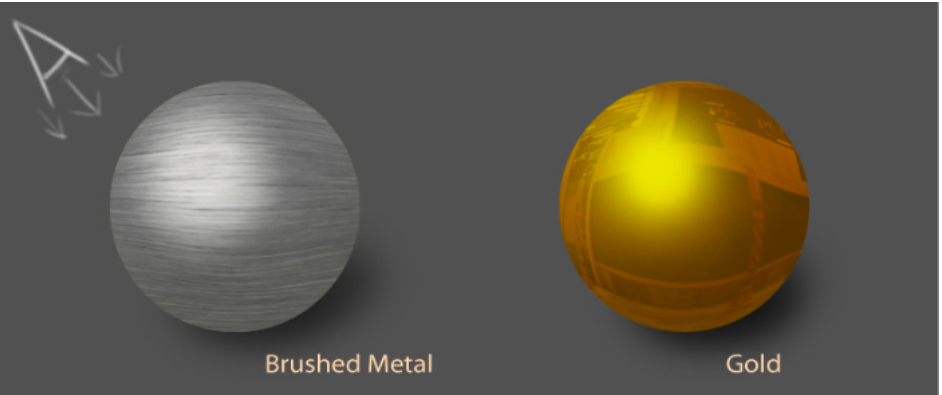
\includegraphics[width=.5\linewidth]{specularbrdf}
\end{figure}
\begin{itemize}
\item[Phong Model]\hfill\\
In the Phong model the specular reflection  has the \textbf{same} angle $\theta$ as the incoming ray with respect to the \textbf{normal} vector, but oriented in the \textbf{opposite} direction, positioned on the same plane as the light and the normal vectors.
\begin{figure}[H]
  \centering
  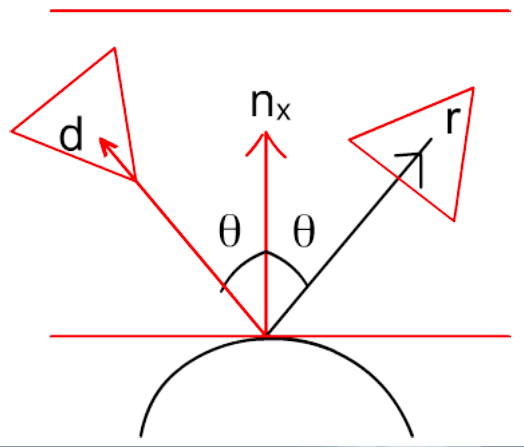
\includegraphics[width=.5\linewidth]{phong}
\end{figure}
Vector $\omega_r$ points in the direction from which the object is being observed in the BRDF. So depending on the type of projection  :
\begin{itemize}
\item \textbf{parallel} projections : rays are all parallel to $\omega_r$  so its a \textbf{constant}
\item \textbf{perspective} projections : $\omega_r =\frac{c-x}{|c-x|} $ , where c is the center of projection and x the point on the surface.
\end{itemize}
The Phong model computes first the angle $\alpha$ between the reflecting direction r and the direction $\omega_r$
\begin{figure}[H]
  \centering
  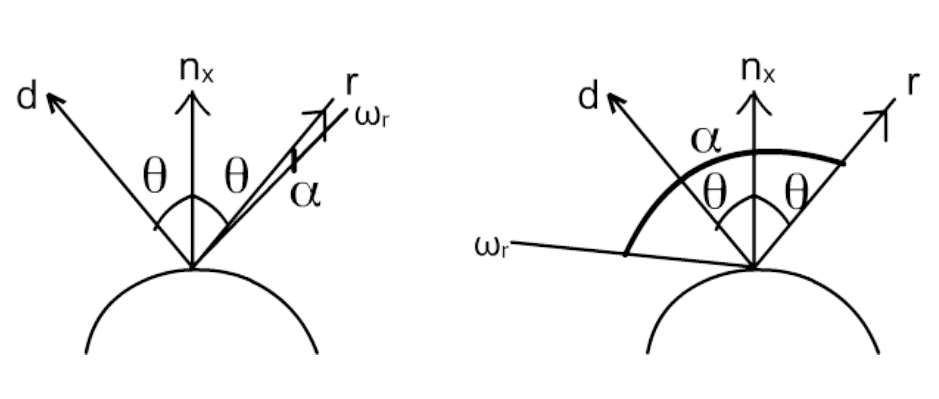
\includegraphics[width=.5\linewidth]{phong2}
\end{figure}
The greater angle $\alpha$ is the less the reflection will be seen : again it is proportional to $cos\alpha$. \\
To create more contained highlight regions , the term $cos\alpha$ is raised to the power of $\gamma$ : 
$$ cos^{\gamma}\alpha$$
The greater is $\gamma$ the \textbf{smaller} is the highlight and the more \textbf{shiny} the object appears
\begin{figure}[H]
  \centering
  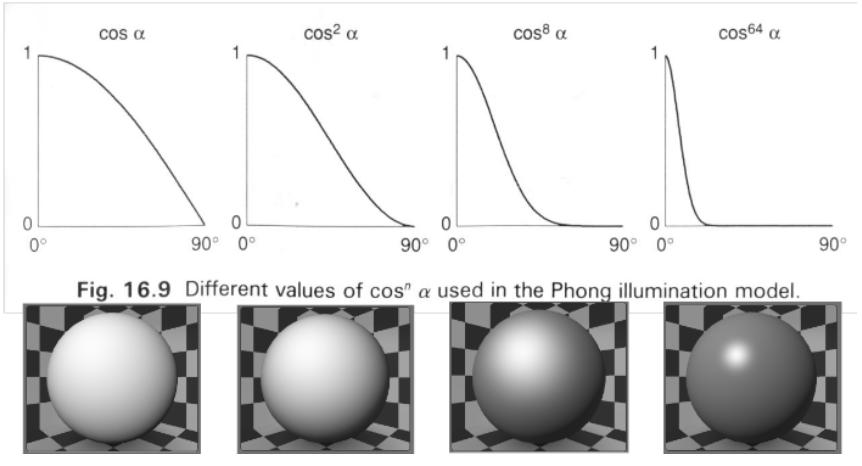
\includegraphics[width=.5\linewidth]{phong3}
\end{figure}
To compute the \textbf{direction} of the \textbf{reflected ray} :
\begin{enumerate}
\item compute $n' = n_x\cdot (d \cdot n_x)$ 
\begin{figure}[H]
  \centering
  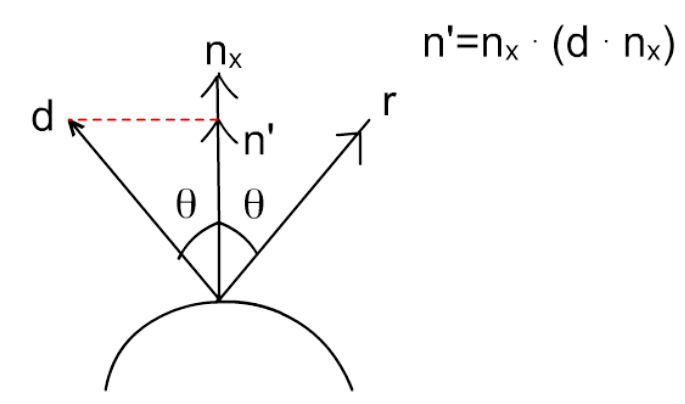
\includegraphics[width=.5\linewidth]{reflectedray1}
\end{figure}
\item compute $d-n'$ to obtain the perpendicular from d to n
\item subtract $(d-n')$ \textbf{two times} to obtain the reflected vector r
\begin{figure}[H]
  \centering
  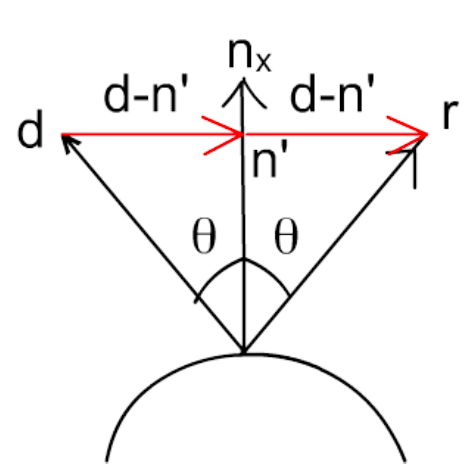
\includegraphics[width=.3\linewidth]{reflectedray2}
\end{figure} 
\end{enumerate}

\[
\boxed{r = d-2(d-n_x \cdot (d \cdot n_x)) = 2n_x \cdot (d \cdot n_x)-d}
\]
Or using the \textbf{rendering notation}:
\[
\boxed{r_{l,x}= 2n_x\cdot (\overrightarrow{\text{xl}} \cdot n_x) - \overrightarrow{\text{xl}}}
\]
When using \textbf{shaders} there is a build-in function called \texttt{reflect(d,n)} that automatically computes the reflection ray given the normal and the light direction.\\
The \textbf{intensity} of the specular reflection can be computed as:
\[
\boxed{COS^{\lambda}\alpha =clamp(\omega_r \cdot \textbf{r})^{\lambda} }
\]
where \textbf{r} is the reflected ray and $\omega_r$ is the direction from which the observer is looking raised at the power of $\gamma$ (the greater $\gamma$  the smaller the reflection highlight ( as seen already above).\\
In summary we  have :
\begin{itemize}
\item $r_{l,x}= 2n_x \cdot (\overrightarrow{\text{lx}} \cdot n_x) - \overrightarrow{\text{lx}}$
\item $f_{\text{specular}}(x, \overrightarrow{\text{lx}},\omega_r) = m_s \cdot \text{clamp}(\omega_r \cdot r_{l,x})^{\gamma}$
where $m_s$ is the specular component color.
\end{itemize}
\item[Blinn Model]\hfill\\
The Phong model is quite \textbf{complex} to compute: to obtain the reflection ray a lot of steps are required. The Blinn model obtains this reflection ray in an alternative way by trying to \textbf{approximate} it. \\
The Blinn model uses \textbf{half-vector h } , which is the vector in the middle of $ d \text{ and } \omega_r$. The angle $\alpha'$ between $n_x \text{ and } h$ is the \textbf{approximation} of the angle $\alpha$ between the \textbf{observer} and the \textbf{reflected ray}.\\
Half vector h can be computed as $$ h_{l,x} = \frac{\overrightarrow{\text{lx}+\omega_r}}{|\overrightarrow{\text{lx}} + \omega_r|} $$ which leads to following color formula :
\[
\boxed{f_{\text{specular}}(x,\overrightarrow{\text{lx}},\omega_r)= \textbf{m}_S \cdot \textbf{clamp}(n_x \cdot h_{l,x})^{\gamma}}
\]
\begin{figure}[H]
  \centering
  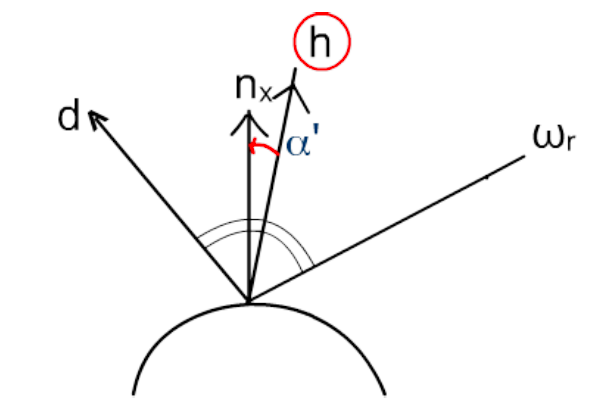
\includegraphics[width=.4\linewidth]{blinn1}
\end{figure}
\item[Blinn vs Phong]\hfill\\
\begin{itemize}
\item Phong , in the end, is \textbf{less} complex than Blinn as Blinn requires a \textbf{normalization} which is more expensive than a \textbf{reflection}.
\item Blinn is better if $d \text{ and } \omega_r$ are constant ( like in parallel projections with directional lights and fixed camera) : this way \textbf{h} is also constant in the entire scene making this model more efficient than the Phong one.
\end{itemize} 
The two techniques are different and lead to different results. This is why almost always \textbf{both} methods are implemented and the final model is chosen depending on the scene that must be reproduced.
\end{itemize}


